% Accessible APA 7 Beamer Presentation Template
% Author: Lanie Molinar Carmelo
% Template Version: 1.0.4 (2025-10-20)
% License: MIT License - https://opensource.org/licenses/MIT
%
% ACCESSIBILITY NOTES:
% - Uses semantic structure (sections, frames) not visual formatting
% - Presenter notes accessible via \note command
% - Color-independent design (no color-only cues)
% - Screen reader compatible with tagged PDF
%
% Usage: Fill in metadata, write content, and build with 'make presentation'
% NOTE: This template uses biblatex with the biber backend.
%       Compile with LuaLaTeX for best results and font support.

% !TeX root = presentation.tex

\DocumentMetadata{
  lang=en-US,
  pdfversion=1.7,
  pdfstandard=ua-1,
  testphase={phase-III}
}

\documentclass[
  12pt,
  aspectratio=169,  % 16:9 widescreen (use 43 for 4:3)
  t,                % Top-align content (change to 'c' for center)
  ignorenonframetext % Ignore text outside frames for article mode
]{beamer}

% ===== THEME AND APPEARANCE =====
% Use a simple, accessible theme with clear structure
\usetheme{default}
\usecolortheme{default}

% Remove navigation symbols (not useful for screen readers)
\setbeamertemplate{navigation symbols}{}

% Use simple footline with page numbers
\setbeamertemplate{footline}[frame number]

% Simple itemize/enumerate (semantic, not decorative)
\setbeamertemplate{itemize items}[circle]
\setbeamertemplate{enumerate items}[default]

% Clear block structure
\setbeamertemplate{blocks}[default]

% ===== FONTS =====
% For maximum compatibility, use system fonts that are typically available
% Times New Roman for text (matches APA paper template)
% Liberation Sans (open-source Arial alternative) for slides
\usepackage{fontspec}
\setmainfont{Times New Roman}
% Use Liberation Sans if available, fallback to Latin Modern Sans
\IfFontExistsTF{Liberation Sans}{
  \setsansfont{Liberation Sans}
}{
  \setsansfont{Latin Modern Sans}  % Fallback for Beamer slide text
}
\usepackage{unicode-math}
\setmathfont{Latin Modern Math}

% Keep fonts readable
\setbeamerfont{title}{size=\Large,series=\bfseries}
\setbeamerfont{frametitle}{size=\large,series=\bfseries}
\setbeamerfont{framesubtitle}{size=\normalsize}

% ===== LANGUAGE AND CITATIONS =====
\usepackage[american]{babel}
\usepackage{csquotes}
\usepackage[style=apa,backend=biber,sortcites=true,sorting=nyt]{biblatex}
\DeclareLanguageMapping{american}{american-apa}
\addbibresource{references.bib}

% ===== ACCESSIBILITY AND METADATA =====
\usepackage{hyperref}
\hypersetup{
  pdftitle={Session 2: The Life of Jesus and the Four Gospels},
  pdfauthor={Lanie Molinar},
  pdfsubject={New Testament},
  pdfkeywords={APA, Beamer, Accessibility, Presentation, Academic, Template,
  Colorado Christian University, Bible, New Testament, Jesus, Gospels},
  pdflang={en-US},
  colorlinks=true,
  linkcolor=blue,
  citecolor=blue,
  urlcolor=blue,
  bookmarksnumbered=true,
  pdfstartview=Fit
}

% ===== NOTES AND HANDOUT CONFIGURATION =====
% Conditional compilation for different output modes
\ifdefined\handoutmode%
  % Handout mode: 4 slides per page, no overlays
  \PassOptionsToClass{handout}{beamer}
  \AtBeginDocument{%
    \usepackage{pgfpages}
    \pgfpagesuselayout{4 on 1}[letterpaper,landscape,border shrink=5mm]
  }
\fi

\ifdefined\withnotes%
  % Notes mode: show notes below slides
  \setbeameroption{show notes}
\else
  % Default: no notes shown
  \setbeameroption{hide notes}
\fi

% ===== PRESENTATION METADATA =====
\title{The Life of Christ and the Four Gospels}
\subtitle{A Journey Through Jesus's Ministry and His Presentation in Scripture}
\author{Lanie Molinar}
\institute{Colorado Christian University}
\date{October 21, 2025}

% ===== DOCUMENT STRUCTURE =====
\begin{document}

% ===== TITLE FRAME =====
\begin{frame}
  	itlepage
  \note{
    Welcome everyone! My name is Lanie Molinar, and today we’ll explore the life and ministry of Jesus Christ and how He is presented in the four gospels. This presentation is designed for middle school students, so feel free to ask questions as we go.
    Duration: 30 seconds.
  }
\end{frame}

% ===== OUTLINE =====
\begin{frame}{Outline}
  \tableofcontents
  \note{
    This slide shows the main topics we’ll cover today. We’ll start by looking at where Jesus ministered, then explore how each gospel writer presents Him. We’ll also discuss what Jesus taught and did, and how He fulfilled the Old Covenant. At the end, I’ll share references and answer any questions you have. Feel free to ask questions at any time!
    Duration: 1 minute.
  }
\end{frame}

% ===== Where Did Jesus Minister? =====
\section{Where Did Jesus Minister?}

\begin{frame}{Geographical Context}
  \framesubtitle{Regions of Jesus's Ministry}

  \begin{figure}
    \centering
  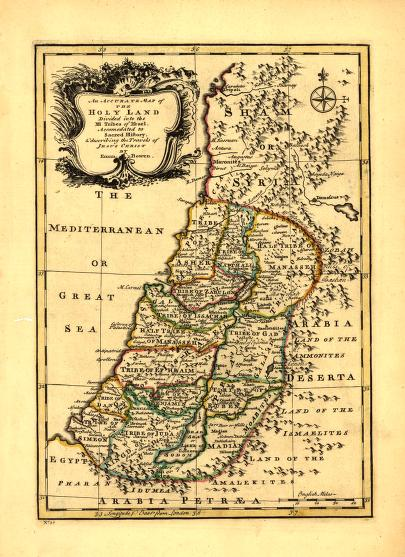
\includegraphics[width=0.8\textwidth]{images/israel-map.jpg}
  \caption{Map of Galilee, Judea, and Samaria, showing Jesus’s ministry regions and tribal divisions. Adapted from \textcite{bowenAccurateMapHoly}}
  \end{figure}

  \note{
  According to \textcite{elwellEncounteringNewTestament2022}, Jesus (see Chapter 8)
    ministered first in Galilee, then moved toward a Phoenician region near
    Tyre. He later traveled to Judea, including Jerusalem, and also ministered
    in Perea across the Jordan River. This map shows these regions and the
    tribal divisions of Israel.
  Duration: 2--3 minutes.
  }
\end{frame}

\begin{frame}{Research Question}

  \begin{block}{Central Question}
    What is the main research question or problem being addressed?
  \end{block}

  \pause%

  \begin{itemize}
    \item Why this question matters
    \item Current gaps in knowledge
    \item Expected contributions
  \end{itemize}

  \note{
    State the research question clearly.
    Explain its significance.
    Discuss what makes this question important or timely.
    Duration: 2 minutes.
  }
\end{frame}

% ===== SECTION 2: LITERATURE REVIEW =====
\end{document}
